\documentclass{amcs}

\usepackage[T2A]{fontenc}
\usepackage[utf8]{inputenc}

%Полезные математические пакеты
\usepackage{amsthm}
\usepackage{amsmath}
\usepackage{amsfonts}
\usepackage{amssymb}

%%% Графика %%%
\usepackage{graphicx}
\DeclareGraphicsExtensions{.pdf,.png,.jpg}

%%% Тексты программ %%%
\usepackage{listings}
\lstset{
  breaklines=true,
  numbers=left,
  numberstyle={\scriptsize},
  showstringspaces=false,
  tabsize=4,
 }

\begin{document}

\bibliography{LaTex_L2}

\newcommand{\vect}[1]{\boldsymbol{\mathbf{#1}}}

\setcourse{Доклад}
\settitle{Теорема Гаусса}
\setstudent{503}{Гаусс К.}
\setsupervisor{ст. преп. кафедры ПМиИ}{Великодный В. И.}
\setchair{ПМиИ}{Кафедра прикладной математики и информатики}{доц.}{Коровай А. В.}
\maketitlepage

\begin{abstract}
  В статье кратко изложены сведения о теореме Гаусса --- важной и полезной <<Штуке>>.
\end{abstract}

\tableofcontents

\ssection{Введение}

\emph{Теорема Гаусса (закон Гаусса)} --- один из основных законов электродинамики, входит в систему уравнений Максвелла. Выражает связь (а именно равенство с точностью до постоянного коэффициента) между потоком напряжённости электрического поля сквозь замкнутую поверхность произвольной формы и алгебраической суммой зарядов, расположенных внутри этой поверхности, деленной на электрическую постоянную $\varepsilon_0$. Применяется отдельно для вычисления электростатических полей. Как было показано в \cite{Tito2017,Gold1987} ...
Аналогично \cite{Pozdnyakov2006}
В работе \cite{Feenstra1995}
Авторы работы \cite{Yoon2005} показали
В \cite{Yutani1996,Tito2017,Yoon2005}
В \cite{Yoon2005}
В \cite{Penner1999}



Теорему Гаусса можно записать для:
\begin{itemize}
\item{электрической индукции}
\item{магнитной индукции}
\end{itemize}

Рассмотрим только первый случай.

\begin{figure}[ht!]
\centering
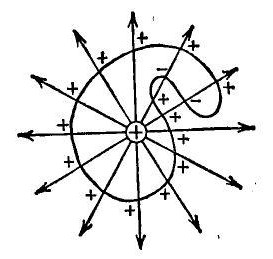
\includegraphics[width=60mm]{L2_p1.jpg}
\caption{Поток вектора через замкнутую поверхность \label{figCurves}}
\end{figure}

\section{Формула для электрической индукции}
\subsection{Интегральная форма}
Для поля в диэлектрической среде электростатическая теорема Гаусса может быть записана в виде (\ref{eq:gauss_int}).
\begin{equation} \label{eq:gauss_int}
\Phi_{\vect{D}}\equiv\oint_S\vect{D}d\vect{S}=4\pi Q.
\end{equation}
\begin{center}
\begin{tabular}[t]{|p{16em}|p{16em}|}
\hline
СГС & СИ \\
\hline
\(\Phi_{\vect{D}}\equiv\oint_S\vect{D}d\vect{S}=4\pi Q\) & \(\Phi_{\vect{D}}\equiv\oint_S\vect{D}d\vect{S}=Q\) \\
\hline
\end{tabular}
\end{center}

\subsection{Дифференциальная форма}
В дифференциальной форме:
\begin{equation} \label{eq:gauss_diff}
\operatorname{div}\vect{D}\equiv\nabla\cdot\vect{D}=4\pi\rho,
\end{equation}

Все выражения записаны для единиц в системе СГС. За подробностями обращайтесь к \cite{b0}.

\section{Дивергенция}
В выражении (\ref{eq:gauss_diff}) используется дивергенция. Это векторный оператор, определяемый следующим образом:
\begin{equation} \label{eq:div_vec}
\operatorname{div}\vect{A}=\nabla\vect{F}=\lim_{n \to \infty}\frac{\Phi_F}{V},
\end{equation}

где $\Phi_F$ --- поток векторного поля.

В декартовых координатах:
\begin{equation} \label{eq:div_dec}
\operatorname{div}\vect{F}=\frac{\partial F_x}{\partial x}+\frac{\partial F_y}{\partial y}+\frac{\partial F_z}{\partial z}.
\end{equation}

\ssection{Заключение}


%\begin{thebibliography}{99}
%\bibitem{LL} Ландау, Л.Д., Лифшиц Е.М. Электродинамика сплошных сред. --- М.:Физматлит, 2005.
%\end{thebibliography}

%\bibliographystyle{gost780s} % ГОСТ 7.80
%\bibliography{L2} % MachLearn.bib

% Приложение
\appendix

\section{Приложение}
\begin{lstlisting}[language=Python]

\end{lstlisting}

\end{document} 